%Author: Siddhesh Wani
%Date: January 7, 2016




\documentclass[12pt]{article}
\usepackage{tikz}
\usetikzlibrary{shapes.geometric, arrows}
\usepackage{hyperref}
\usepackage[a4paper]{geometry}
%DO NOT EDIT start
%Define different shapes to be used in flowchart
\tikzstyle{startstop} = [rectangle, rounded corners, minimum width=3cm, minimum height=1cm,text centered, draw=black, fill=red!30]
\tikzstyle{io} = [trapezium, trapezium left angle=70, trapezium right angle=110, minimum width=3cm, minimum height=1cm, text centered, draw=black, fill=blue!30]
\tikzstyle{process} = [rectangle, minimum width=3cm, minimum height=1cm, text centered, draw=black, fill=orange!30]
\tikzstyle{decision} = [diamond, minimum width=3cm, minimum height=1cm, text centered, draw=black, fill=green!30]
\tikzstyle{arrow} = [thick,->,>=stealth]
\tikzstyle{connector} = [signal,draw=black,fill=olive!30]%,text width=1cm,text height=1.5cm,align=center]
%DO NOT EDIT end




\begin{document}
\newgeometry{top=2cm, bottom=0.5cm,right=1cm,left=1.5cm}

\vspace*{2cm}
\begin{center}

\section*{\hypertarget{AST_GetASTFile}AST\_GetASTFile.sci}
{Siddhesh Wani}\\
 
\end{center}


\textbf{Introduction}\\
Gets next function from `FileInfo' structure and calls `SciFile2ASTFile' with appropriate arguments to generate AST file file from scilab file.

\begin{center}

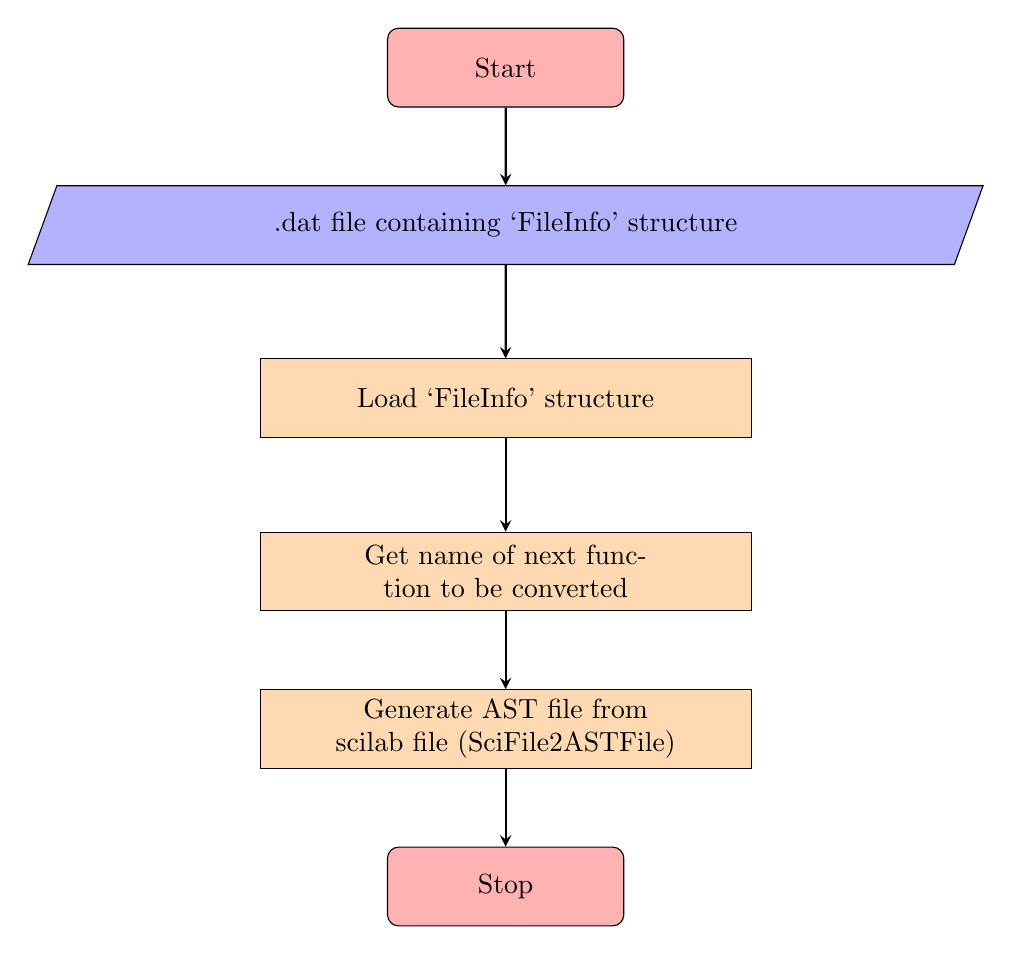
\begin{tikzpicture}[node distance=2cm]
\node (start) [startstop, xshift=-4cm] {Start};
\node (input) [io, below of=start, text width=6cm]{.dat file containing `FileInfo' structure};
\node (fileinfo)[process, below of=input, text width=6cm, yshift=-0.2cm]{Load `FileInfo' structure};
\node (nextfun) [process, below of=fileinfo, text width=6cm, yshift=-0.2cm]{Get name of next function to be converted};
\node (ast)[process, below of=nextfun, text width=6cm]{Generate AST file from scilab file (SciFile2ASTFile)};
\node (stop)[startstop, below of=ast]{Stop};

\draw [arrow] (start) -- (input);
\draw [arrow] (input) -- (fileinfo);
\draw [arrow] (fileinfo) -- (nextfun);
\draw [arrow] (nextfun) -- (ast);
\draw [arrow] (ast) -- (stop);


\end{tikzpicture}
\end{center}

\end{document}